\documentclass[10pt]{article}
\usepackage[margin=0.72in]{geometry}
\usepackage[T1]{fontenc}
\usepackage{lmodern}
\usepackage{microtype}
\usepackage{amsmath,amssymb}
\usepackage{enumitem}
\usepackage{booktabs}
\usepackage{graphicx,hyperref}
\setlength{\parskip}{3pt}
\setlength{\parindent}{0pt}
\setlist{nosep,leftmargin=*}
\title{\vspace{-1.2em}ICT 5143 Capstone Evaluation Report — Problem 6\\
\large Fair Allocation of Job Training under Uncertain Treatment Benefits}
\author{Akshay Wali (261090830018) \and Mohit Das (261090840018)}
\date{}
\begin{document}
\maketitle
\section{Research question and contribution}
Does requiring evidence of nonnegative incremental earnings in every audited race group change policy feasibility at fixed training capacity? The comparison isolates the group-benefit floor and the lower confidence bound within the tested candidate class.

\section{Data and causal model}
The primary data are the Dehejia--Wahba experimental NSW subset (185 treated, 260 randomized controls; $n=445$), with real 1978 earnings as the outcome. Recorded race/ethnicity indicators and age define intersectional groups. The male-only sample does not support gender fairness analysis. Overlap and hidden-confounding stress tests use separate simulations.

The causal DAG contains baseline demographics and covariates, randomized treatment receipt $T$, and earnings $Y$. Identification uses randomization, consistency, positivity and no interference. The primary estimand is
\[
V(\pi)=E[\pi(X)\{Y(1)-Y(0)\}],\quad
B_g(\pi)=E[\pi(X)\{Y(1)-Y(0)\}\mid G=g].
\]
Actual treatment receipt $T$ is distinct from hypothetical allocation $D=\pi(X)$. Policy value is evaluated with doubly robust scores. A separate discrete Bayesian network checks factor operations, evidence handling, variable elimination, and clique-tree inference.

\section{Methods and experiments}
Five outer folds each contain 267 development, 89 validation, and 89 test participants. Baselines include random allocation, predicted-earnings ranking, treatment-benefit ranking, shallow policy trees, and equal-rate allocation. We compare unconstrained selection, a nonnegative point-estimate group-benefit floor, and a nonnegative lower-confidence-bound (LCB) floor. Target capacities are 20\%, 40\%, and 60\%.

\section{Results}
The experimental mean difference was 1,794.34 (95\% CI [518.53, 3,132.21]). Adjusted outcome regression estimated 1,676.34 (95\% CI [448.12, 2,997.58]). Constant-propensity IPW reproduced the experimental difference. At 40\% capacity, benefit ranking exceeded predicted-earnings ranking by an estimated 394.98 per eligible participant, with a paired 95\% interval of [$-110.36$, 856.59].

\begin{table}[htbp]
\centering
\caption{Feasibility and held-out value at 40\% capacity. Value is incremental earnings per eligible participant.}
\begin{tabular}{lrrr}
\toprule
Rule & Original folds & Fold refits & Held-out value\\
\midrule
Unconstrained & 5/5 & 500/500 & 1,074.67\\
Point-estimate floor & 2/5 & 158/500 & Unavailable\\
LCB floor & 0/5 & 0/500 & Unavailable\\
\bottomrule
\end{tabular}
\end{table}

At 40\% training capacity, the lower-confidence-bound rule selected a feasible policy in 0 of 5 original outer folds and 0 of 500 development-sample fold refits. The refitting study held the validation and test participants fixed. Because no rule was selected in the original folds, the full-sample held-out policy value was unavailable. The point-estimate rule selected policies in two original folds, and one met the 200-unit validation utility tolerance. The unconstrained method completed all 100 five-fold refit repeats, while both constrained methods completed zero.

\begin{figure}[htbp]
\centering
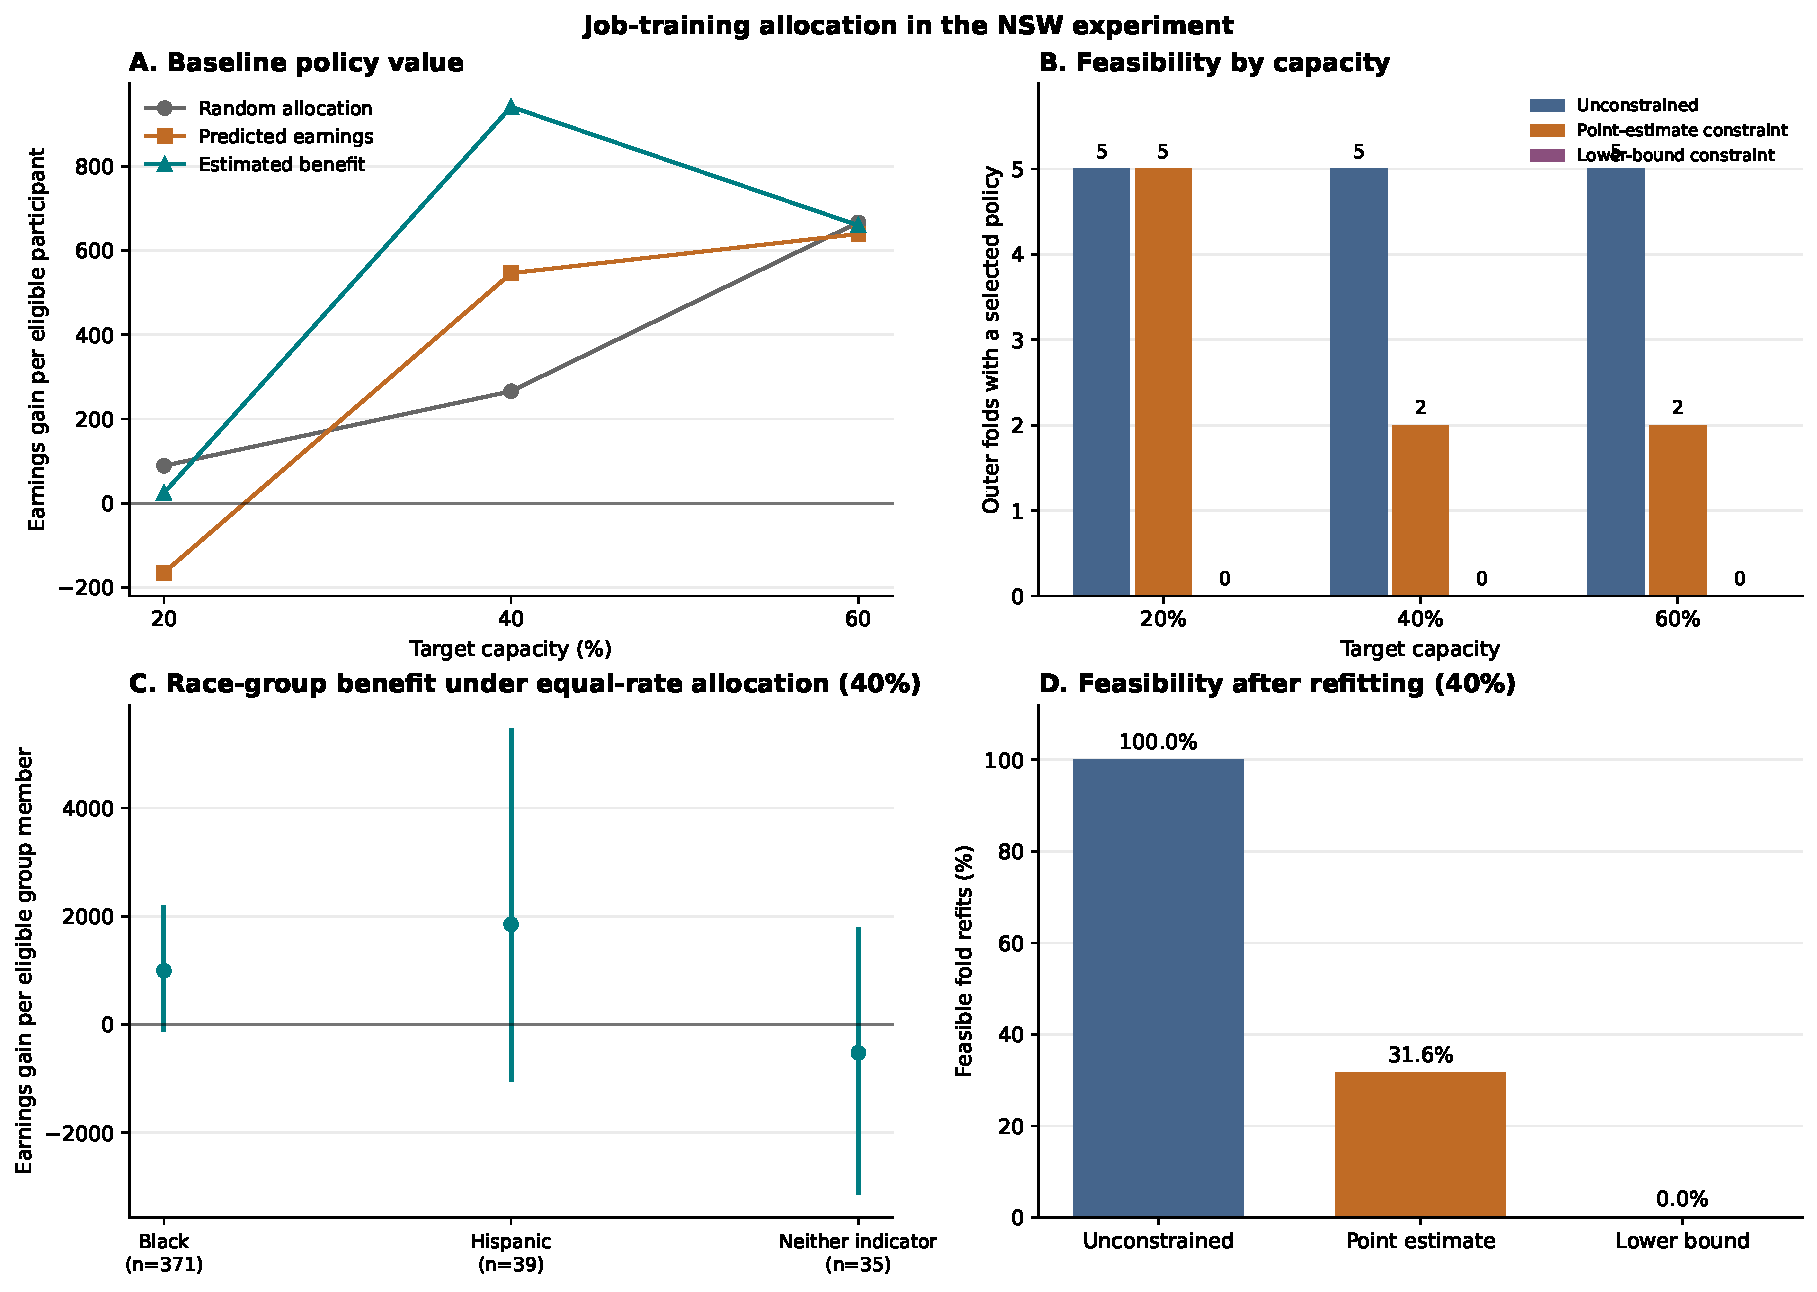
\includegraphics[width=\linewidth,height=0.48\textheight,keepaspectratio]{results/figures/nsw_main_results.pdf}
\caption{NSW policy results. Panels B and D show feasibility. A zero bar indicates zero feasible selections. At 40\% capacity, the lower-confidence-bound rule selected a feasible policy in 0 of 5 original outer folds and 0 of 500 development-sample fold refits. Its full-sample held-out policy value was unavailable. Panel C shows fixed-policy bootstrap intervals.}
\end{figure}

\section{Robustness and reproducibility}
At 40\% capacity, both the raw-trained and transformed-trained LCB rules selected zero of five policies. Evaluated on raw earnings, unconstrained value was 1,074.67 for raw training and 911.36 for training on $\operatorname{asinh}(\mathrm{RE78}/1000)$. In the weak-overlap simulation, clipping at 0.01 reduced policy-value RMSE from 758.76 to 625.49, while clipping at 0.05 increased it to 880.39.

Variable elimination and clique-tree inference agreed across six diagnostic queries, with a maximum absolute discrepancy of $5.55\times10^{-17}$. The full pipeline completed in a fresh Windows Python 3.14 environment. SHA-256 comparisons matched exactly for the ATE estimates, constraint selections, outer-fold summary, and refitting summary.

\section{Limitations}
The feasibility finding applies to the tested candidate rules, audited groups, group floor, and uncertainty procedure. Sparse group denominators limit interpretation of outcome-conditioned fairness gaps. The historical, male-only sample limits generalization. The known-effect and hidden-confounding simulations address mechanisms under their respective data-generating assumptions.

\section*{References}
\small
\begin{enumerate}[label={[\arabic*]}]
\item LaLonde (1986), ``Evaluating the Econometric Evaluations of Training Programs with Experimental Data,'' \emph{AER} 76(4), 604--620.
\item Dehejia \& Wahba (1999), ``Causal Effects in Nonexperimental Studies,'' \emph{JASA} 94(448), 1053--1062.
\item Pearl (2009), \emph{Causality}, 2nd ed., Cambridge University Press.
\item Kitagawa \& Tetenov (2018), ``Who Should Be Treated?'' \emph{Econometrica} 86(2), 591--616.
\item Athey \& Wager (2021), ``Policy Learning with Observational Data,'' \emph{Econometrica} 89(1), 133--161.
\item Kim \& Zubizarreta (2023), ``Fair and Robust Estimation of Heterogeneous Treatment Effects for Policy Learning,'' ICML, PMLR 202, 16997--17014.
\item Joshi, Zhang \& Bareinboim (2024), ``Towards Safe Policy Learning under Partial Identifiability,'' \emph{AAAI} 38(12), 13004--13012.
\item Kock \& Preinerstorfer (2026), ``Regularizing Fairness in Optimal Policy Learning with Distributional Targets,'' \emph{Journal of Econometrics} 254(B), 106186.
\end{enumerate}
\end{document}
